% DO NOT COMPILE THIS FILE DIRECTLY!
% This is included by the other .tex files.

\begin{frame}
\titlepage
\end{frame}

\begin{frame}
  \frametitle{MISP and CIRCL}
  \begin{center}
    
\includegraphics[scale=0.45]{circl.png}
    \hspace{2.5em}
    
\includegraphics[scale=0.35]{misp.pdf}
  \end{center}
  \begin{itemize}
    \item CIRCL is mandated by the Ministry of Economy and acting as the Luxembourg {\bf National CERT for the private sector}. 
    \item CIRCL runs multiple large MISP communities performing {\bf active daily threat-intelligenge sharing}
    \item CIRCL leads the development of {\bf MISP and many other open source softwares}\footnote{AIL-Framework, D4-project, CVE-search, passive-(ssl/dns), lookyloo}.
  \end{itemize}
\end{frame}


\begin{frame}
  \frametitle{The aim of this presentation}
  \begin{itemize}
     \item Provide a quick intro what MISP is and what issues we try to tackle
     \item A small update of what has happened around MISP's development over the past year
     \item Where we're headed from here
  \end{itemize}
\end{frame}

\section{Intro on MISP}

\begin{frame}
\frametitle{Objectives of MISP}
\begin{itemize}
       \item MISP is a {\bf threat information sharing} platform that is free \& open source software
       \item A tool that {\bf collects} information from partners, your analysts, your tools, feeds
       \item Normalises, {\bf correlates}, {\bf enriches} the data
       \item Allows teams and communities to {\bf collaborate}
       \item {\bf Feeds} automated protective tools and analyst tools with the output
\end{itemize}
\end{frame}

\begin{frame}
\frametitle{MISP Features Highlights}
    \begin{itemize}
        \item Extensive Rest {\bf API}
        \item Automatic {\bf correlation}
        \item Granular distribution levels and {\bf synchronisation} systems
        \item A wide range of {\bf ingestion systems}
        \item {\bf Visualisation tools} for dashboarding, graphing, statistics
        \item A host of {\bf export formats}, covering a wide range of use-cases
        \begin{itemize}
            \item {\bf IDSes / IPSes}: \texttt{Suricata, Bro/Zeek, Snort}
            \item {\bf SIEMs}: \texttt{CEF, STIX}
            \item {\bf Host scanners}:  \texttt{OpenIOC, STIX, CSV, Yara}
            \item {\bf Analysis tools}: \texttt{Maltego}
            \item {\bf DNS policies}: \texttt{RPZ}
        \end{itemize}
    \end{itemize}
\end{frame}

\section{High level overview of the past year's changes}

\begin{frame}
  \frametitle{MISP's evolution since the last AusCERT}
  \begin{itemize}
    \item Since the AusCERT 2019 (31/05/2019) we've had:
    \begin{itemize}
        \item 34 releases
        \item 4398 commits
        \item 97 contributors contributing to the core software and its components
    \end{itemize}
    \item COVID-19 didn't negatively impact the progress made all that much
  \end{itemize}
\end{frame}

\begin{frame}
  \frametitle{So what were the main changes?}
  \begin{itemize}
     \item Loads of {\bf bug fixes}
     \item A host of improvements to how MISP behaves in general
     \item {\bf Security fixes}, including several CVEs (keep your MISP up to date!)
     \item {\bf Internal tuning} for better scaling and performance altogether
     \item Massively expanding {\bf context libraries}
     \item Several major features (let's talk about these)
  \end{itemize}
\end{frame}

\section{Major features since last year}

\begin{frame}
\frametitle{Timelining in MISP}
\begin{itemize}
	\item The goal was to capture activity timelines
        \item All attributes and objects can have first-seen/last-seen data       
\end{itemize}
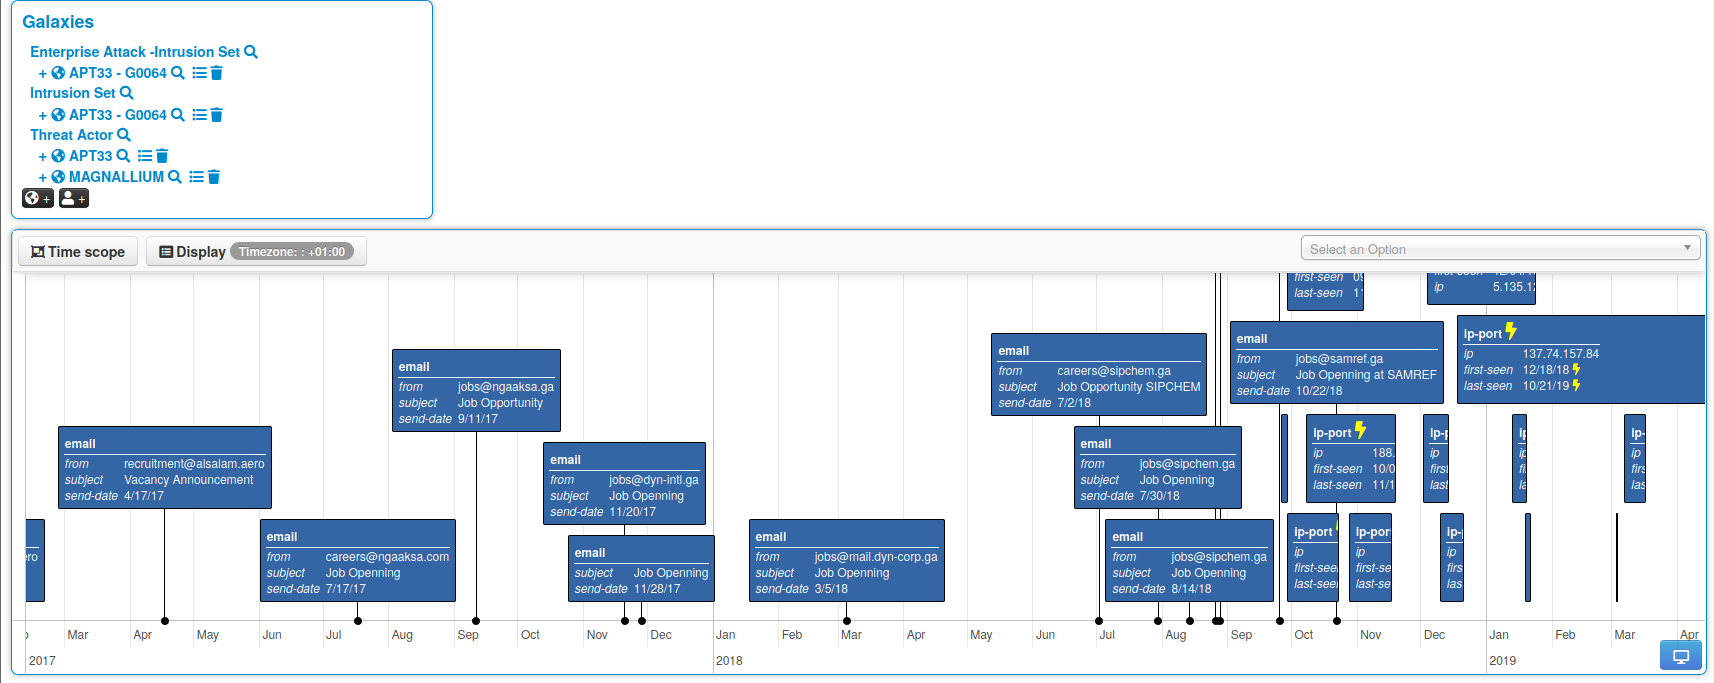
\includegraphics[scale=0.25]{images/timeline.png}
\end{frame}

\begin{frame}
\frametitle{Timelining in MISP}
\begin{itemize}
	\item Why is this interesting?
        \item {\bf IoC lifecycle management} is one of the biggest challenges we face
        \item Timeline information allows us to better {\bf express a story}, rather than {\bf share dumps of IoCs}
        \item {\bf Time-based correlation} of certain actions helps us understand an incident
\end{itemize}
\end{frame}

\begin{frame}
\frametitle{Dashboarding}
\begin{itemize}
	\item Outcome of our personal initiatives to track the COVID-19 spread
        \item New built-in {\bf dashboarding system} directly available in MISP
        \item Dashboard widgets are modular and {\bf easy to build}
        \item Create widgets that are {\bf ACL aware}
        \item The COVID-19 MISP community turned out to be a massive success
        \begin{itemize}
             \item Just register if you would like to have access at \url{https://covid-19.iglocska.eu}
        \end{itemize}
        \item COVID-19 use-cases are just an example though (admin widgets, trend widgets, gamification, etc)
\end{itemize}
\end{frame}

\begin{frame}
\frametitle{Dashboarding}
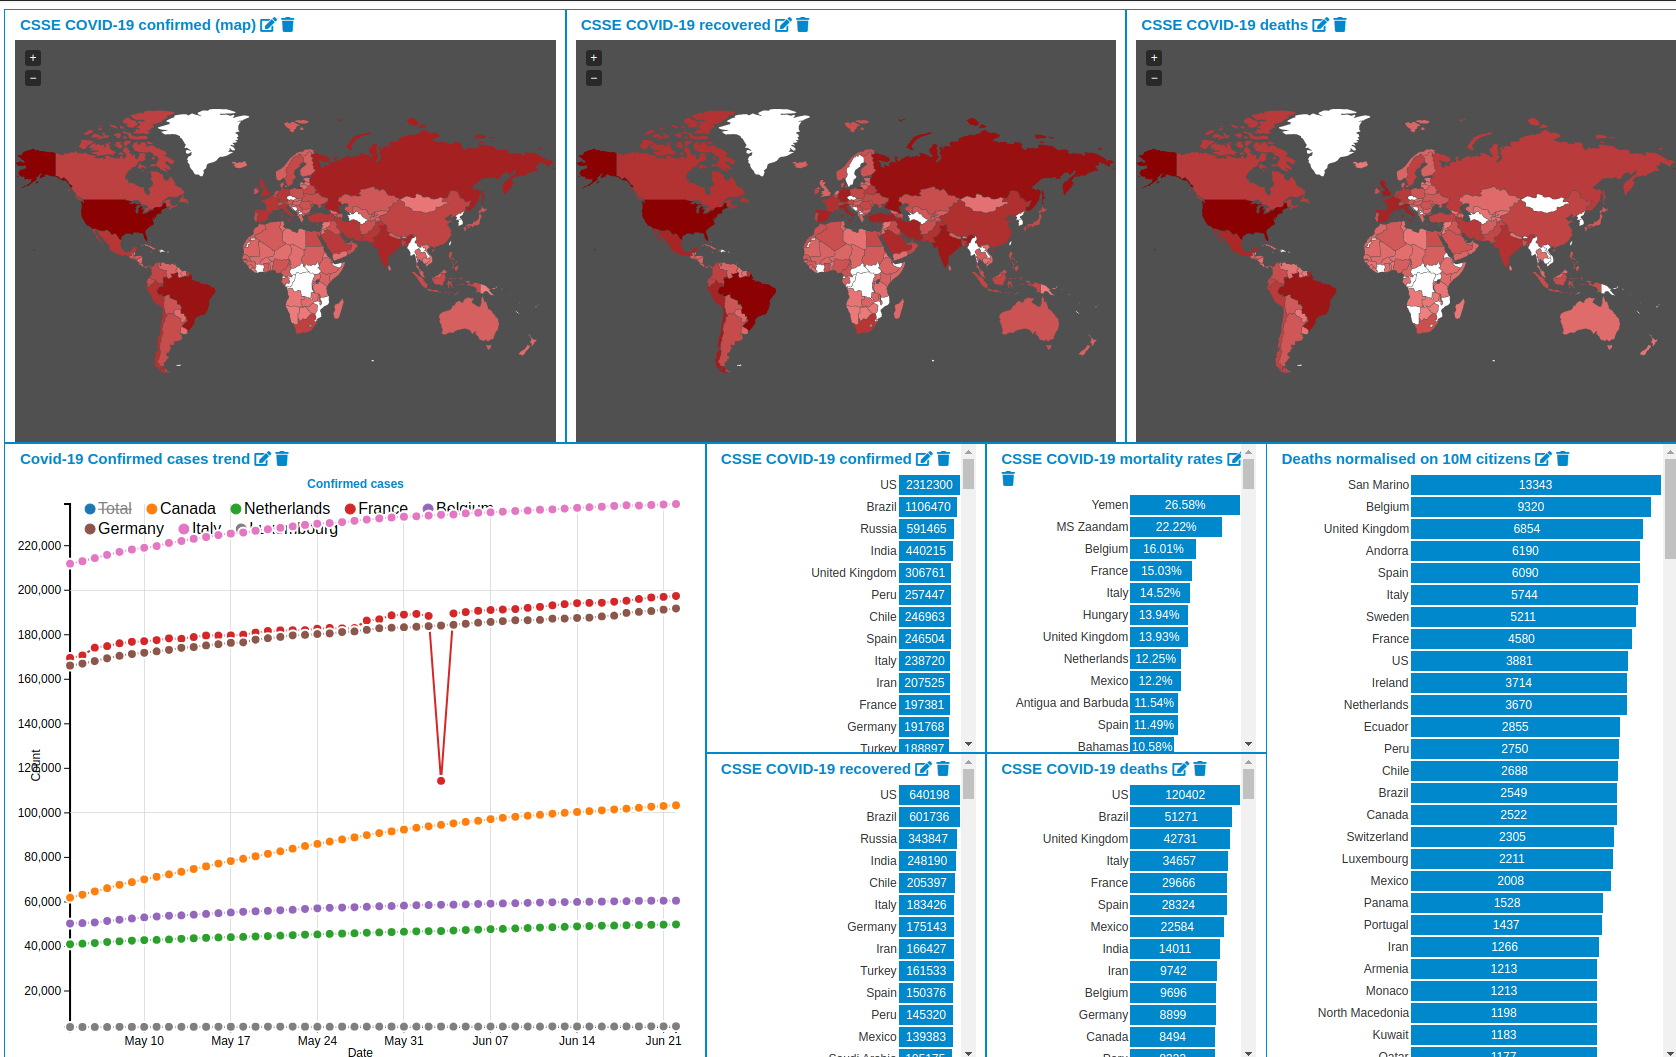
\includegraphics[scale=0.25]{images/dashboard.png}
\end{frame}


\begin{frame}
\frametitle{Decaying indicators v2}
\begin{itemize}
        \item Further improvement on our indicator {\bf life-cycle management} tool
	\item {\bf User settings} are now taken into account when crafting queries
        \item {\bf Tool specific} user accounts can be pre-configured with decaying settings
        \item {\bf Taxonomy} numerical values can be re-mapped to fit internal needs
        \item {\bf Sightings} factor into the decay scores
\end{itemize}
\end{frame}

\begin{frame}
\frametitle{Convert attributes to objects}
\begin{itemize}
    \item Allow users to easily select a set of attributes and automatically propose suitable object templates
\end{itemize}
\begin{center}
    \movie[width=9cm,height=6cm]{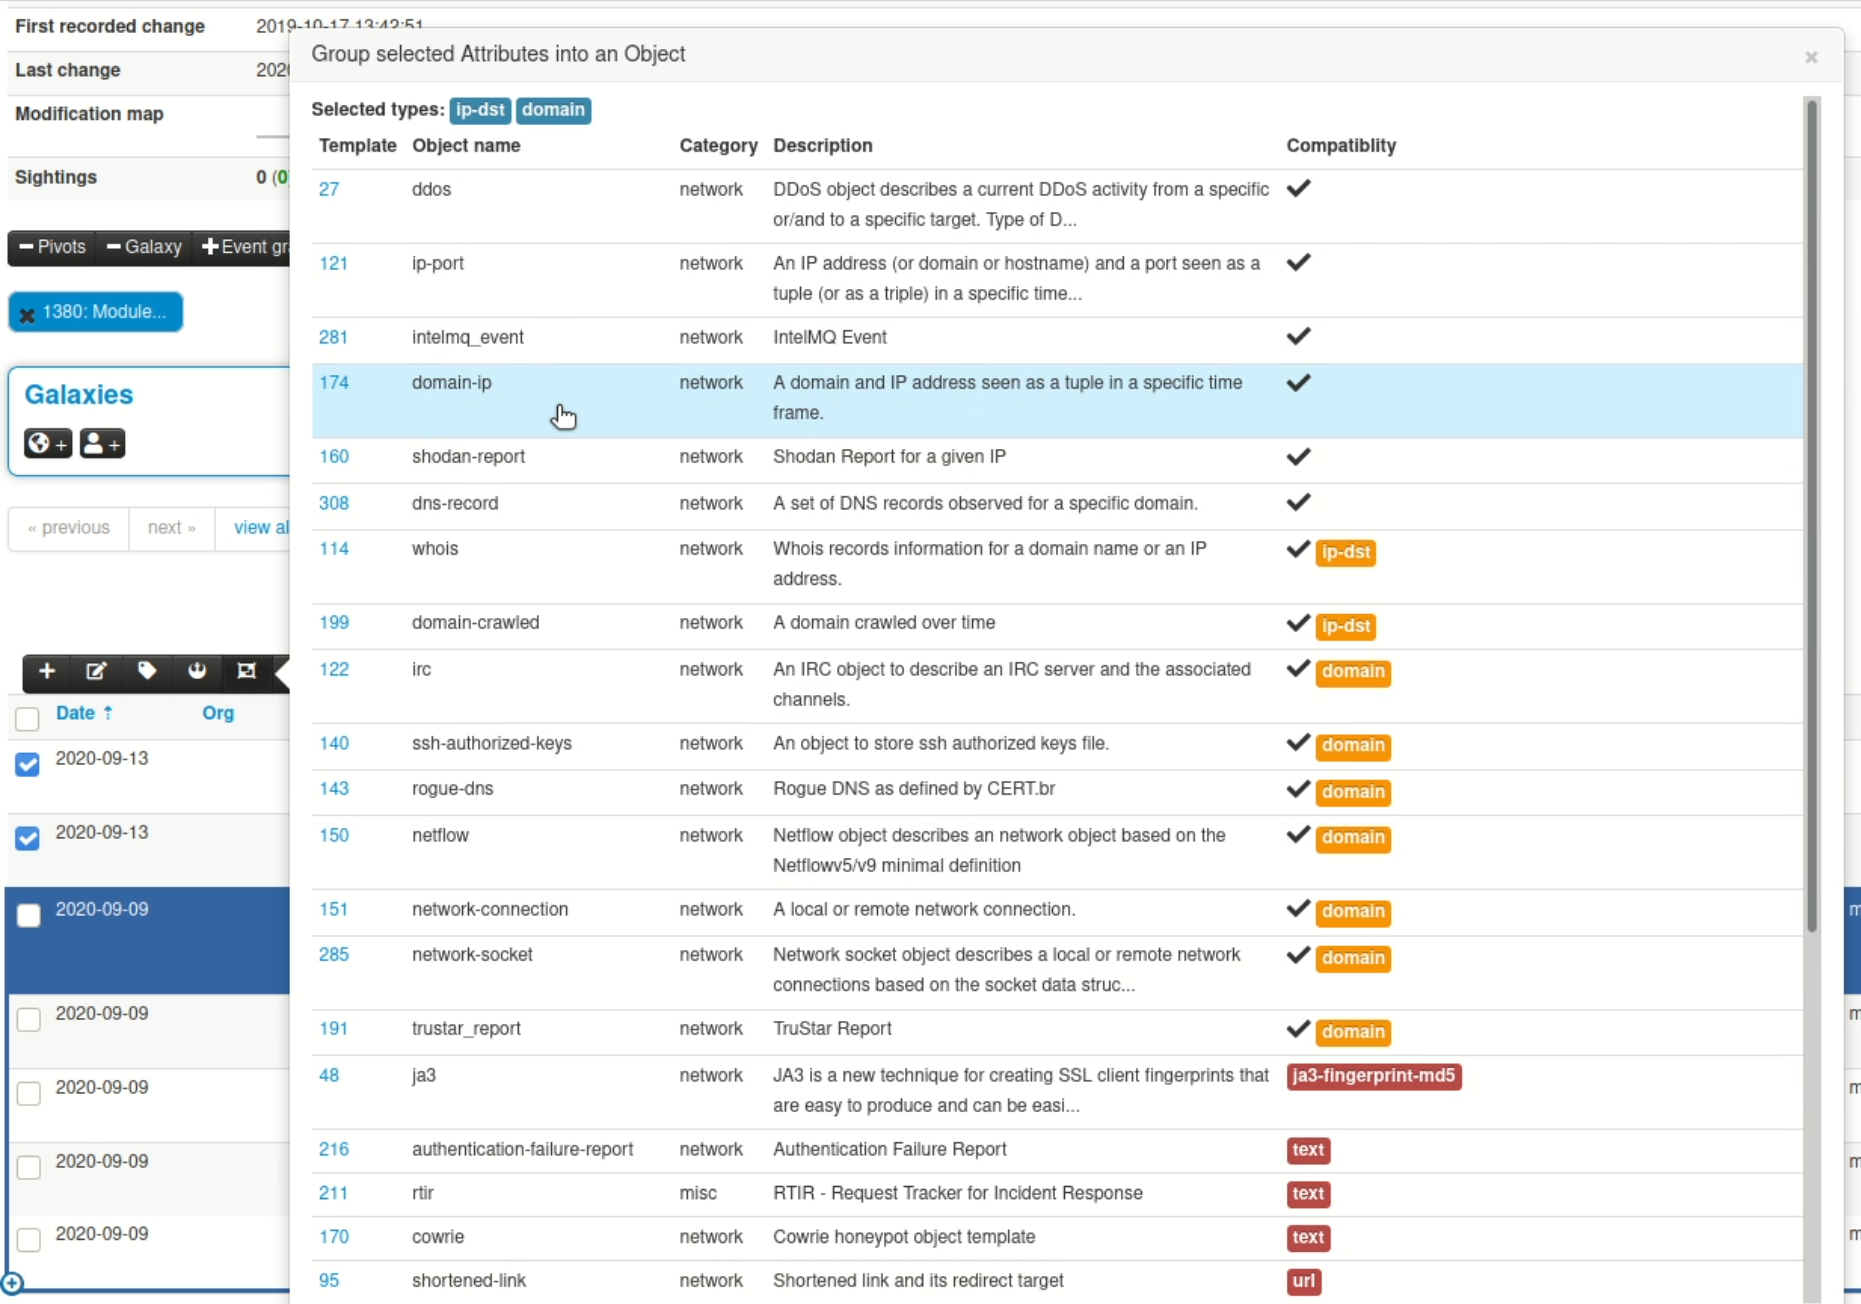
\includegraphics[scale=0.13]{attributes_to_object.png}}{attributes_to_object.mp4}
\end{center}
\end{frame}

\begin{frame}
\frametitle{Massive rewrite of PyMISP}
\begin{itemize}
	\item Python 3.6+ is a minimum since the modern PyMISP rework
        \item Use of {\bf objects} with a {\bf long list of helpers} allows for easy creation/modification of MISP data
        \item PyMISP's {\bf CI testing} suite has grown massively, allowing us to catch more and more issues as we commit changes
        \item Automated testing {\bf including synchronising} several MISP instances
\end{itemize}
\end{frame}

\begin{frame}
\frametitle{Community management improvements}
\begin{itemize}
	\item {\bf User configurations} - manage per user rule sets to alter MISP's behaviour ({\bf alerting rules}, {\bf dashboard configuration}, etc)
        \item {\bf Community listings} - to help users find the right communities and negotiate access
        \item Various improvements to authorization systems - {\bf E-mail based OTP}, {\bf further integrations with SSO systems}
\end{itemize}
\end{frame}

\begin{frame}
\frametitle{Integrations}
\begin{itemize}
	\item Long list of {\bf integrations}, both via our export system and module systems and by other tools integrating with MISP
        \item Continuous iterations of our connectors using other formats (a massive STIX 2 rework has just dropped)
        \item Integrations with analysis tools, such as with {\bf Maltego}
        \item Tighter integration with other {\bf OSS frameworks we develop in-house} (AIL, D4)
        \item Mapping of libraries to taxonomies/galaxies/object templates
        \item ATT\&CK like matrices from other domains (disinformation via AMITT, various sectorial groups)
\end{itemize}
\end{frame}

\begin{frame}
\frametitle{MISP format modules}
\begin{itemize}
    \item Initial modules
    \begin{itemize}
        \item Return {\bf single attributes} only
        \item As {\bf light-weight} as possible
        \item Good to handle {\bf simple queries}
    \end{itemize}
    \item MISP format modules
    \begin{itemize}
        \item Return {\bf MISP standard format}
        \item {\bf Backward compatible}
        \item Much better results with {\bf complex data}
    \end{itemize}
\end{itemize}
\pause
\begin{itemize}
    \item Why are they interesting?
    \pause
    \item Keep the {\bf context} of the results returned by the modules
    \item {\bf Validation} of the data to ingest
\end{itemize}
\end{frame}

\begin{frame}
\frametitle{MISP format modules}
\begin{center}
    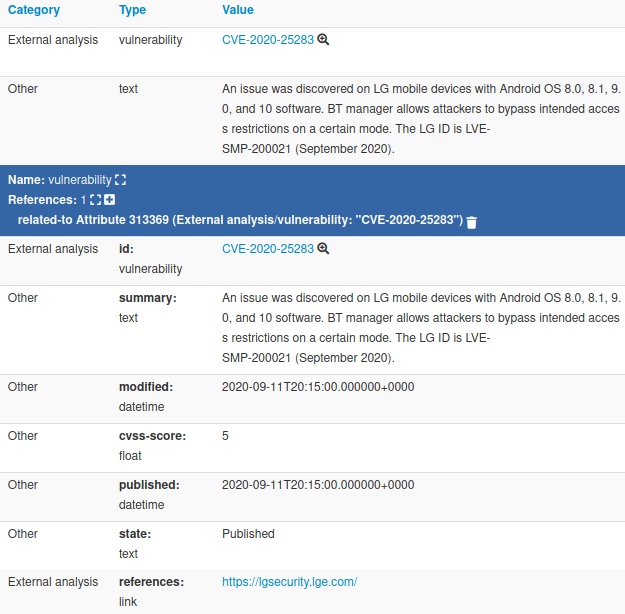
\includegraphics[width=0.7\linewidth]{cve_module.png}
\end{center}
\end{frame}

\section{The road ahead}

\begin{frame}
\frametitle{So that's where we are now}
\begin{itemize}
	\item Let's have a brief look at what is on our immediate and long-term roadmaps
        \item For the long-term ones, priorities shift rapidly
\end{itemize}
\end{frame}

\begin{frame}
\frametitle{Going further with the MISP modules}
\begin{itemize}
    \item Move the export modules to the {\bf built-in export library}
    \item Enable import modules to be able to {\bf generate entire events}
    \item {\bf Expansion modules} for the event scope
\end{itemize}
\begin{itemize}
    \item Move the modules to {\bf background processes} with a
messaging system
    \item Avoid the results preview when applicable
    \begin{itemize}
        \item Preview page can be very heavy
        \item Difficulty is {\bf dealing with uncertain results} (without the user
having final say)
    \end{itemize}
\end{itemize}
\end{frame}

\begin{frame}
\frametitle{MISP galaxy 2.0}
\begin{itemize}
	\item MISP galaxies will be fully managed via MISP directly
        \item Create, modify, {\bf share your custom galaxies} with the usual sync / ACL mechanisms
        \item Fork and {\bf provide your own perspective} to already existing knowledge-base items
        \item Build {\bf relationships between galaxy clusters} (Threat actor A uses Tool B and targets Sector C)
        \item Already available in beta
\end{itemize}
\end{frame}

\begin{frame}
\frametitle{Reports}
\begin{itemize}
	\item Create {\bf markdown reports} and share them along with your events
        \item Structured information is great for automation, but sometimes plain prose helps telling a story
        \item Shared along with events, distribution per report item configurable
\end{itemize}
\end{frame}

\begin{frame}
\frametitle{Community management at scale}
\begin{itemize}
	\item {\bf Cerebrate} is a new OSS frameworks that we're building
        \item Manage {\bf organisation, sharing group, encryption key} data for communities
        \item {\bf Instrument} MISP instances and the interconnectivity between them via Cerebrate
        \item Introduce {\bf information signing} by validating signatures / ownership via trusted Cerebrate nodes
        \item Early alpha already available
\end{itemize}
\end{frame}

\begin{frame}
\frametitle{Rework of the MISP internals}
\begin{itemize}
	\item We are planning on moving MISP to a {\bf more modern stack} (cake4/bs4)
        \item Cerebrate also acts as a {\bf test-bed} for this move and relies on MISP internals that have already been ported
        \item We have been silently {\bf reworking a lot of the internals} of MISP to make the migration possible (UI generator systems for example)
\end{itemize}
\end{frame}

\section{Conclusion}

\begin{frame}
  \frametitle{To sum it all up...}
  \begin{itemize}
     \item Many interesting things are happening
     \item We are following {\bf several routes} of development (internal improvements, contextualisation, integrations, operational improvements, community building)
     \item We have many more ideas, but sadly days are only 24 hours long
     \item There are {\bf many ways to get involved}
     \item Prioritisation is hard. {\bf Let us know what you think we should focus on}!
  \end{itemize}
\end{frame}

\begin{frame}
  \frametitle{Get in touch if you have any questions}
  \begin{itemize}
    \item Contact CIRCL
    \begin{itemize}
      \item info@circl.lu
      \item \url{https://twitter.com/circl_lu}
      \item \url{https://www.circl.lu/}
    \end{itemize}
    \item Contact MISPProject 
    \begin{itemize}
      \item \url{https://github.com/MISP}
      \item \url{https://gitter.im/MISP/MISP}
      \item \url{https://twitter.com/MISPProject}
    \end{itemize}
    \item Join the COVID-19 MISP community
    \begin{itemize}
      \item \url{https://covid-19.iglocska.eu}
    \end{itemize}
  \end{itemize}
\end{frame}
